%!tex engine=xelatex
\documentclass[a4paper]{article}
\usepackage[margin=1.2in]{geometry}
\usepackage{amssymb,amsmath}
\usepackage{fontspec}
\setmainfont{EB Garamond}

\usepackage{aastexmacros}
\usepackage{hyperref}
\usepackage{natbib}
\bibliographystyle{unsrtnat}

\newcommand{\defn}[1]{\emph{#1}}

\title{Brushtail: Extracting Meaningful Features from Faraday Spectra}
\author{
    M. J. Alger\\{\small Research School of Astronomy and Astrophysics, The Australian National University}\\{\small Data61, CSIRO}\\
    C. S. Ong\\{\small Data61, CSIRO}\\{\small Research School of Computer Science, The Australian National University}\\
    N. M. McClure-Griffiths\\{\small Research School of Astronomy and Astrophysics, The Australian National University}\\}

\begin{document}
    \maketitle

    \begin{abstract}
        Early-science data from the Australian Square Kilometre Array Pathfinder (ASKAP) are coming fast. Wide-area radio projects such as the Evolutionary Map of the Universe (EMU) and the Polarisation Sky Survey of the Universe’s Magnetism (POSSUM) already have terabytes of ASKAP observations for use in early-science and survey planning. We have applied unsupervised machine learning methods to learn a meaningful representation of these early-science observations and demonstrated that this representation generalises across different sets of observations. We use this representation to address physical problems such as polarised source characterisation and physical model-fitting. Our approach provides a way to use early-science data even without full understanding of the unique instrumentation effects brought to the table by ASKAP.
    \end{abstract}

    \section{Introduction}

        The Australian Square Kilometre Array (ASKAP) will conduct wide-area radio surveys like the Evolutionary Map of the Universe (EMU) and the Polarised Sky Survey of the Universe's Magnetism (POSSUM). Thanks to ASKAP's 30 square degree field-of-view and high resolution, these surveys will produce a huge amount of radio data in a very short time, and processing it quickly will be difficult. We hope that machine learning algorithms will be able to help us with the data deluge, but we need to train them first. While plenty of data is available almost none of it is labelled, meaning that supervised machine learning approaches won't be directly applicable. We could set up a citizen science website like Radio Galaxy Zoo --- but even crowdsourced manual labelling is a slow and expensive process. One possible approach to applying machine learning is to first learn meaningful features of the polarised radio sky, a process called \defn{representation learning} \citep{bengio12representation}, and then learn mappings from these features. The idea is that representation learning leverages the whole unlabelled dataset to find good features, and then we can use a smaller labelled dataset to learn the mapping we want. Representation learning seems to work well on multitask and transfer problems \citep{bengio12representation}.

        We want to apply a representation learning approach to the POSSUM early-science data to extract meaningful features that are good for a broad variety of purposes and are robust enough to use across multiple POSSUM fields. We train a feature extractor using a simple Faraday screen simulator and using these features train a classifier for Faraday complexity following \citet{brown19complexity}. This classification task provides a test-bed for trialling our unsupervised approach.

        \subsection{Faraday Spectra and Faraday Complexity}

            Radio polarimetry measures the Stokes parameters $I, Q, U,$ and $V$. $V$ represents the circularly polarised component of the radio waves and is generally zero for extragalactic sources. $I$ is the standard `continuum' emission. $Q$ and $U$ represent the linear polarisation and together form a complex polarisation $Q + iU$. $Q + iU$ varies as a function of wavelength $\lambda$. The variation is called \defn{Faraday rotation}, the rotating of polarised light due to magnetic fields. A \defn{Faraday screen} is a magnetic structure that induces a rotation showing up in $Q + iU$ as a linear function of $\lambda^2$. The slope of this line is called the \defn{rotation measure}, measured in rad~m~$^{-2}$. More complicated magnetic structures exist and can be described as the sum of Faraday screens. An observation of a polarised radio source viewed through a magnetic structure that is not a single Faraday screen is called a \defn{Faraday complex} source (as opposed to \defn{Faraday simple}). For these sources, $Q + iU$ is non-linear in $\lambda^2$. Examples of Faraday complex structures include having multiple Faraday screens within one beam, and systems inducing rotation which also emit.

            By taking something very similar to a Fourier transform of $Q + iU$ along $\lambda^2$ we obtain the \defn{Faraday spectrum} $F(\phi)$. $\phi$, measured in rad~m~$^{-2}$, is a scaled Fourier conjugate of $\lambda^2$ and is called the \defn{Faraday depth}. A Faraday simple source has a single peak at a Faraday depth corresponding to the rotation measure of the source: Faraday depth can be viewed a generalisation of the rotation measure to complex sources.

            The Faraday spectrum is complicated by the fact that our observations are sampled at different wavelengths $\lambda$. This means that the observed Faraday spectrum is convolved with a \defn{rotation measure spread function} (RMSF), the Fourier transform of the sampled wavelengths. This is much the same as how radio images are convolved with a point spread function (PSF).

    \section{Deconvolving Autoencoders}

        Inspired by denoising autoencoders, we propose to build a `deconvolving autoencoder' to learn a latent representation of Faraday spectra.

        A autoencoder is made up of an encoder $f_\theta(\cdot)$ and a decoder $g_\vartheta(\cdot)$ parametrised by $\theta, \vartheta$. The goal is to reconstruct $x \in \mathbb{R}^d$, i.e. we have a loss function
        \begin{equation}
            \mathcal L(\theta, \vartheta) = \|x - (g_\vartheta \circ f_\theta)(x)\|^2.
        \end{equation}
        $f_\theta(x)$ is a representation of $x$ and we can use it for other purposes. A modification of this is a \defn{denoising autoencoder} which instead requires reconstructing $x$ from a noisy version $N(x)$:
        \begin{equation}
            \mathcal L(\theta, \vartheta) =  \|x - (g_\vartheta \circ f_\theta)(N(x))\|^2.
        \end{equation}
        This again finds a representation $f(x) \in \mathbb{R}^k$. Usually $k < d$. Note that ideally $f(x) = f(N(x))$, i.e. $f$ can `ignore' or `remove' the noise.

        We suggest a loss function as follows. Denote the RMSF as a vector $r$, and let $\ast$ denote a vector convolution. Let $\Psi(x) = r \ast x$ and $\Psi^\dagger_\varrho(x) = \varrho \ast x$. Let $z = \Psi(x)$. Let $0 \leq \alpha \leq 1$. Then our loss function is:
        \begin{equation}
            \mathcal L(\theta, \vartheta, \varrho) = \alpha\|x - (\Psi^\dagger_\varrho \circ (g_\vartheta \circ f_\theta) \circ \Psi)(x)\|^2 + (1 - \alpha)\|z - (g_\vartheta \circ f_\theta)(z)\|^2
        \end{equation}
        Intuitively, we want to reconstruct an observation $x$ as well as its RMSF-convolved variant $z$. $f_\theta \circ \Psi$ is an encoder with a fixed first operation convolving with the RMSF. $\Psi^\dagger_\varrho \circ g_\vartheta$ is a decoder that necessarily finishes with a convolution over some vector $\varrho$. $g_\vartheta \circ f_\theta$ is itself an autoencoder for convolved spectra. By including this in our loss function $\Psi^\dagger_\varrho$ should be interpretable as an `inverse' to the RMSF convolution, which is of practical interest to radio astronomers. We propose to further constrain $\varrho$ as a linear function of the RMSF, i.e.
        \begin{equation}
            \varrho = r^T W
        \end{equation}
        for some weight matrix $W$.

        % A \emph{deconvolving autoencoder} aims to reconstruct a Faraday spectrum $x$ from $x$ convolved with the RMSF.  Then
        % \begin{align}
        %     x &\approx (\Psi^\dagger \circ (g \circ f) \circ \Psi)(x)\\
        %     z &\approx (g \circ f)(z)
        % \end{align}

        % The loss function is
        % with $0 \leq \lambda \leq 1$.

        \begin{figure}
            \centering
            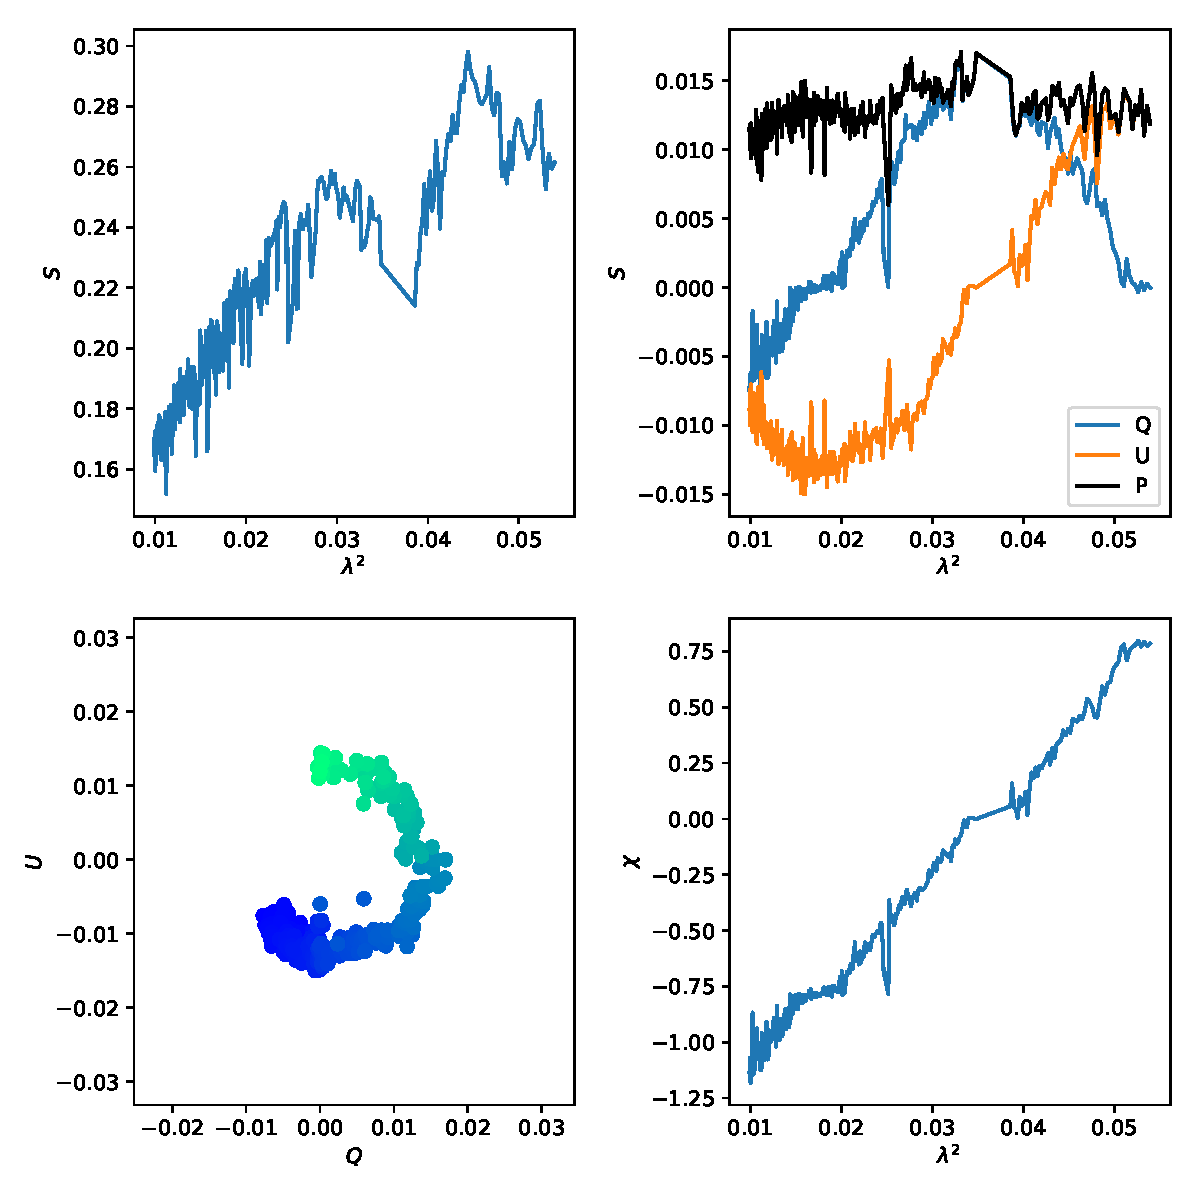
\includegraphics[width=0.9\textwidth]{dae/jack-example.pdf}
            \caption{\label{fig:jack-data} ATCA data courtesy of Jack Livinston.}
        \end{figure}

        \begin{figure}
            \centering
            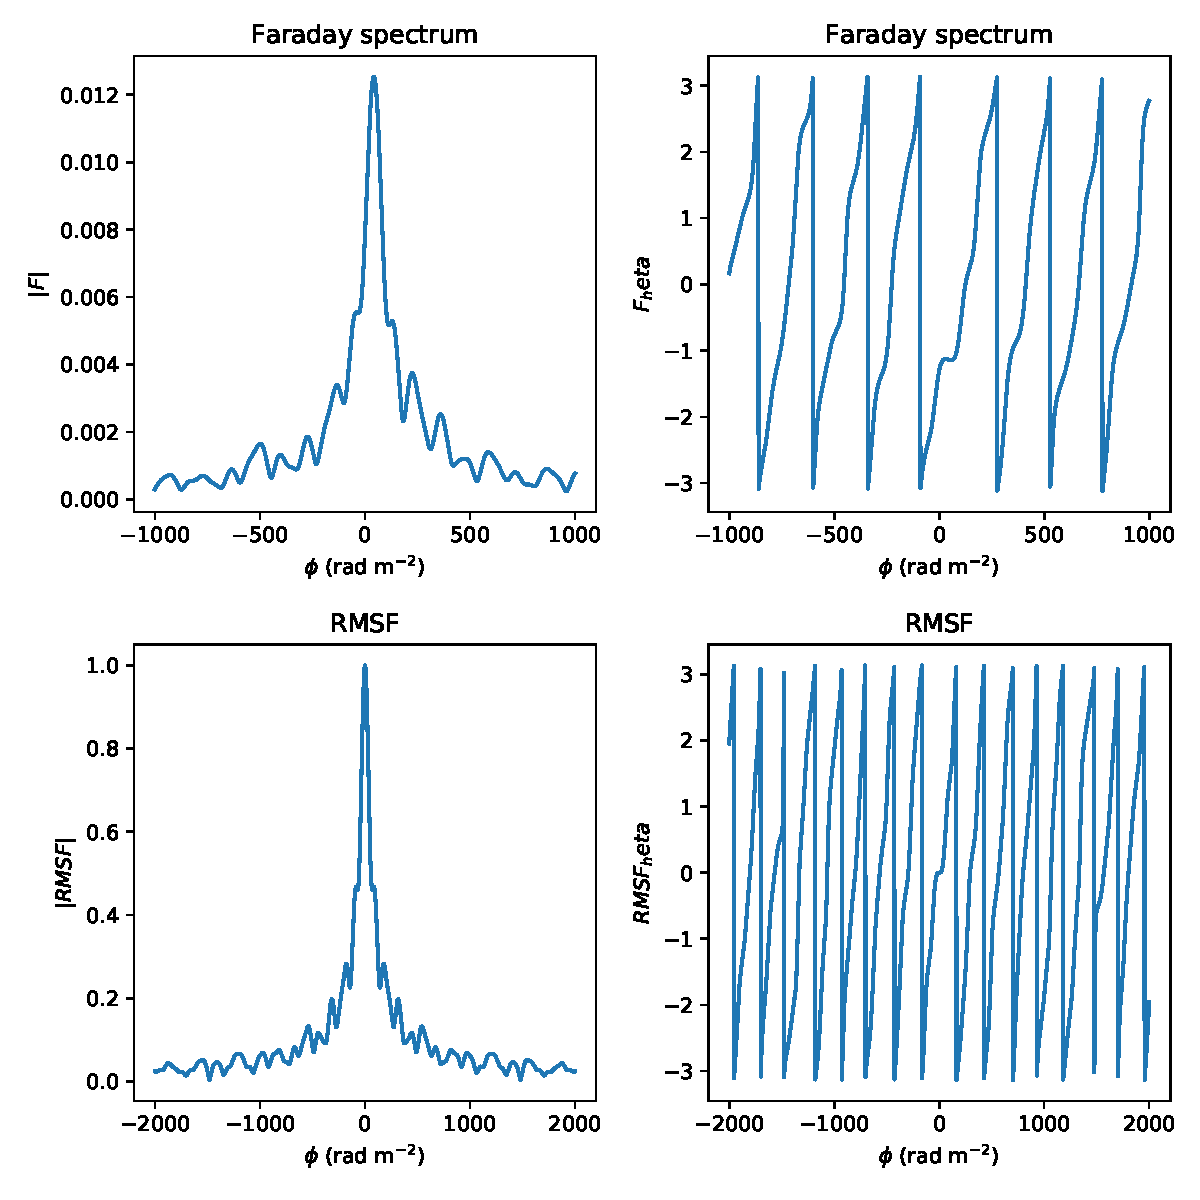
\includegraphics[width=0.9\textwidth]{dae/jack-example-faraday.pdf}
            \caption{\label{fig:jack-faraday} Some of Jack's ATCA data in Faraday space.}
        \end{figure}

    % \section{Experiment 1: Comparing Representations of Simulated Spectra}

    %     \begin{figure}
    %         \centering
    %         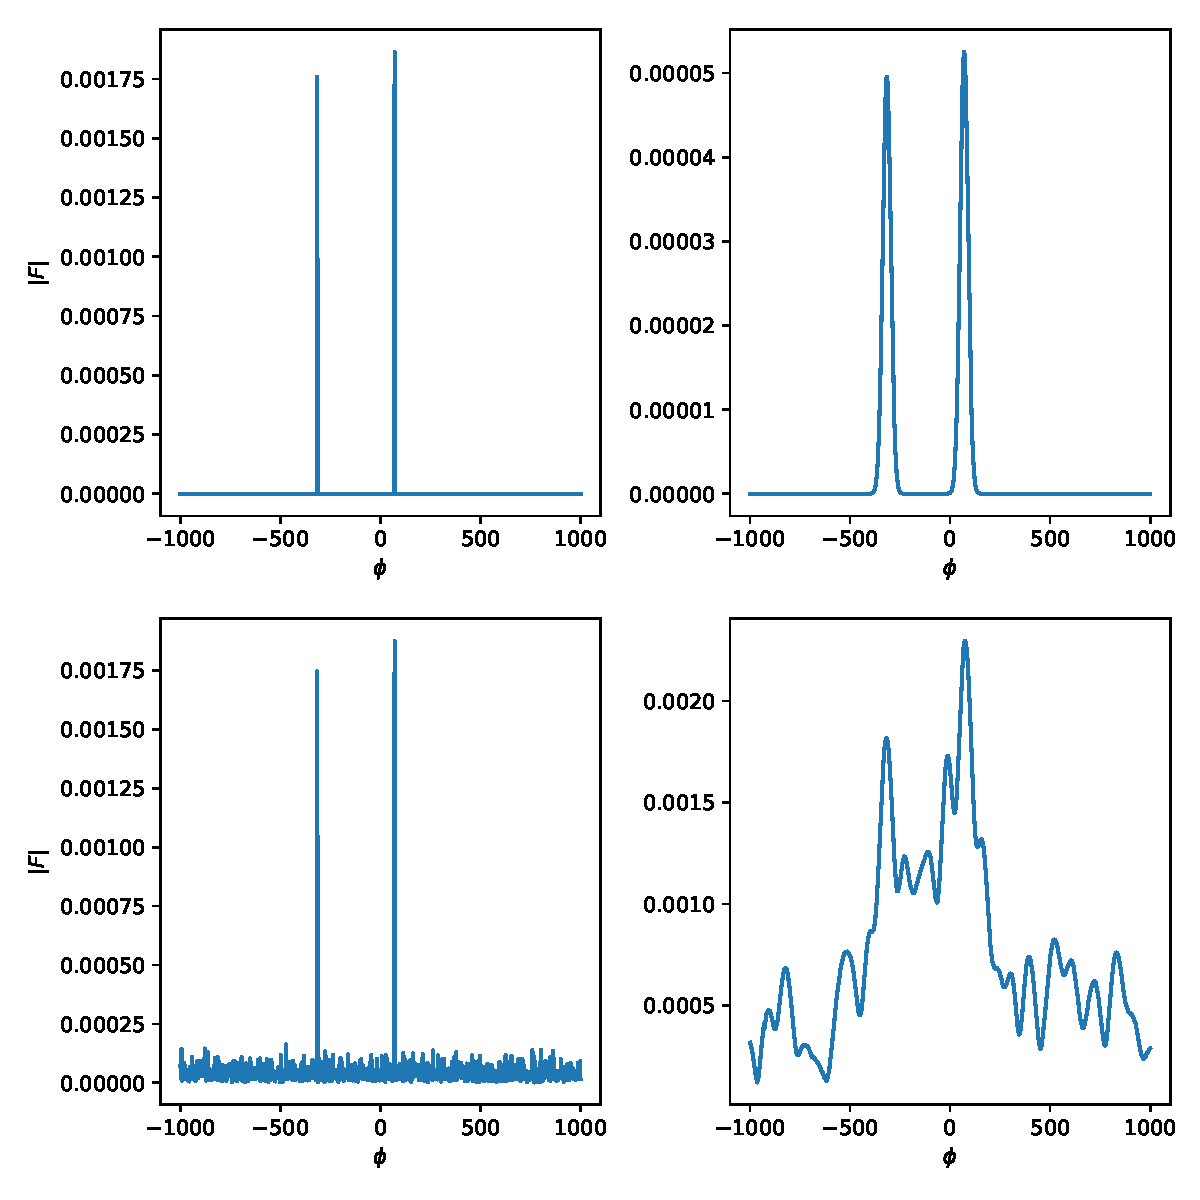
\includegraphics[width=0.9\textwidth]{dae/simulated-screens.pdf}
    %         \caption{\label{fig:simulation} From left-to-right, top-to-bottom: A groundtruth spectrum with two Faraday screens; the groundtruth convolved with a Gaussian; the groundtruth with Gaussian noise; the noisy spectrum convolved with the RMSF.}
    %     \end{figure}

    %     We generated $N \times 2$ Faraday depths $\phi \in [-800, 800]\text{ rad m}^{-2}$ and $N \times 2$ corresponding phases $\psi \in [-\pi, \pi]$. We then generated a `true' spectrum with $1000$ channels in $\phi$, from $-1000$ to $1000\text{ rad m}^{-2}$. To this we added Gaussian noise $\sim \mathcal{N}(0, 5 \times 10^{-5})$ and convolved with a RMSF from Jack Livingston's ATCA observations to get our simulated spectra. We trained a deconvolving autoencoder, autoencoder, denoising autoencoder, and PCA on these spectra.

    %     % We also convolved separately the true spectrum with a Gaussian with width $20\text{ rad m}^{-2}$ to obtain a smoothly-varying target. 

    % \section{Data}

    %     Jack has provided some Faraday spectra from near the galactic centre, shown in \autoref{fig:jack-data} and \autoref{fig:jack-faraday}. There aren't enough to train something, but such a scenario is fairly realistic in polarisation. There isn't often a lot of data! We will train a deconvolving autoencoder (DCAE) on Faraday spectra of simulated two-screen models and then apply it to Jack's data and the S-band Polarization All-Sky Survey (SPASS).

    \section{Principal Curves}

        Assume we have some samples drawn from a 1D curve in a Euclidean 3D ambient space. We parametrise the curve $f(\lambda)$ with $\lambda \in [0, 1]$. The samples are drawn with zero-mean Gaussian noise in the ambient space, so for a data point $y$ generated by the curve at location $\lambda$ we observe
        \begin{equation}
            y = f(\lambda) + \epsilon.
        \end{equation}
        Given a set of such $y$, how can we find $f$? For a particular value $\lambda$, if we take $y_\lambda$ to be the set of all points generated by the curve at $\lambda$, then
        \begin{equation}
            f(\lambda) = \mathbb E[y \mid y \in y_\lambda]
        \end{equation}
        Given a point $y$ and a curve $f$, which $\lambda$ generated $y$? One answer would be the $\lambda$ that minimises $f(\lambda) - y$, i.e. the orthogonal projection of $y$ onto $f$. If we use this approach, then the above equation describes an \emph{self-consistent} curve. Perhaps instead we take a probabilistic approach, and look for $p(\lambda \mid y, f)$. By Bayes rule, this is proportional to $p(y \mid \lambda, f) p(\lambda \mid f)$. But $p(y \mid \lambda, f)$ is just the noise distribution $\epsilon$, and we can assume $p(\lambda \mid f)$ is constant. Then
        \begin{equation}
            f(\lambda) = \mathbb E[y \mid y \in y_\lambda] = \frac{\int_0^1 p(y \mid \lambda, f_0) y\  d\lambda}{\int_0^1 p(y \mid \ell, f_0)\ d\ell}
        \end{equation}
        where $f_0$ is some initial guess.

        todo: write down the iterative algorithm, attempt to show convergence, attempt to show that a doubled-back curve is a local minimum.

    \bibliography{brushtail}

\end{document}